\chapter{Contração muscular e função motora}\label{ch:b2:muscle-movement}

Uma velocista sai do bloco com uma força sobre a pista de três vezes o
seu peso, desenvolvida em um quinto de segundo por músculos que estavam
relaxados um instante antes. Nada na célula encurtou para isso: os
filamentos internos deslizaram uns sobre os outros, puxados por milhões
de mãos moleculares, cada uma dando um passo de dez nanômetros e
soltando, dez vezes por segundo, pagas um ATP de cada vez. Este
capítulo toma a \omterm{def:b2:cell-differentiation:myogenesis}{fibra muscular} construída no \cref{ch:b2:cell-differentiation} e a faz
funcionar: o deslizamento dos filamentos e o motor que os impulsiona, o
interruptor de cálcio que liga e desliga o motor, o comando vindo do
nervo, a mecânica da força e da velocidade, e o modo como o sistema
nervoso gradua o conjunto, de um \omterm{def:b2:muscle-movement:motorunit}{abalo} a um pique de corrida.

\section{Os filamentos deslizantes}

\begin{proposition}[O mecanismo dos filamentos deslizantes]\label{prop:b2:muscle-movement:sliding}
\index{filamentos deslizantes}\index{sarcômero!contração}
Quando uma \omterm{def:b2:cell-differentiation:myogenesis}{fibra muscular} encurta, seus \omterm{def:b2:cell-differentiation:fibre}{sarcômeros} encurtam (\cref{ch:b2:cell-differentiation}),
mas nem os filamentos grossos de miosina nem os filamentos finos de
actina mudam de comprimento: os filamentos finos deslizam para dentro
ao longo dos grossos, a banda I e a zona H se estreitam, e os discos Z se
aproximam. A sobreposição entre os dois conjuntos de filamentos é onde a
força é gerada, e um \omterm{def:b2:cell-differentiation:fibre}{sarcômero} gera força em proporção a essa
sobreposição: a partir de um comprimento distendido de
\qty{3.6}{\micro m}, sem sobreposição e sem força, a força aumenta
linearmente à medida que os filamentos se sobrepõem mais, atinge um
platô perto de \qty{2.2}{\micro m}, onde todas as cabeças de miosina
estão diante da actina, e volta a cair abaixo de \qty{2.0}{\micro m},
quando os filamentos finos colidem entre si e os grossos batem nos
discos Z. O comprimento de repouso de um músculo no corpo fica sobre o
platô --- o que é a primeira pista de como a força é produzida.
\end{proposition}
\begin{proof}[Evidências]
A.~F.~Huxley e Niedergerke, e H.~E.~Huxley e Hanson (1954), mediram as
bandas de fibras isoladas e de \omterm{def:b2:cell-differentiation:fibre}{miofibrilas} isoladas por microscopia de
interferência e de contraste de fase enquanto elas encurtavam: a banda A
conservava seu comprimento e a banda I encolhia, de modo que os
filamentos deslizam. Gordon, Huxley e Julian (1966) mantiveram uma fibra
isolada em comprimentos fixos com um dispositivo de retroalimentação que
mantinha constante o comprimento dos \omterm{def:b2:cell-differentiation:fibre}{sarcômeros} de um segmento, e
verificaram que a força era proporcional à sobreposição entre os
filamentos grossos e finos medida por microscopia eletrônica --- a curva
comprimento--tensão, com seu platô e seus dois ramos lineares,
exatamente como a geometria dos filamentos prevê.
\end{proof}

\begin{omfigure}
\begin{minipage}[b]{0.5\linewidth}\centering
\begin{tikzpicture}[every node/.style={font=\scriptsize}]
  \foreach \y/\lab/\ov in {2.4/{relaxado, \qty{2.6}{\micro m}}/0.9, 1.2/{contraído, \qty{2.0}{\micro m}}/0.3} {
    \begin{scope}[yshift=\y cm]
      \draw[very thick, omThm] (0,-0.35) -- (0,0.35); \draw[very thick, omThm] (4.4-2*\ov+1.0,-0.35) -- (4.4-2*\ov+1.0,0.35);
      \pgfmathsetmacro{\len}{4.4-2*\ov+1.0}
      \foreach \dy in {-0.25,0.05,0.25} { \draw[thick, omDef] (0,\dy) -- (1.5,\dy); \draw[thick, omDef] (\len,\dy) -- (\len-1.5,\dy); }
      \draw[line width=3pt, omExo!80!black] (\len/2-1.1,-0.1) -- (\len/2+1.1,-0.1);
      \node[right] at (\len+0.15,0) {\lab};
    \end{scope}
  }
  \node[align=center] at (2.7,0.1) {os filamentos conservam\\seus comprimentos; a sobreposição\\aumenta à medida que os discos Z\\se aproximam};
\end{tikzpicture}
\end{minipage}\hfill
\begin{minipage}[b]{0.48\linewidth}\centering
\begin{tikzpicture}
\begin{axis}[
  width=\linewidth, height=4.8cm,
  axis x line=bottom, axis y line=left,
  xmin=1.2, xmax=3.8, ymin=0, ymax=1.15,
  xlabel={comprimento do sarcômero (\unit{\micro m})}, ylabel={força (relativa)},
  xlabel style={font=\scriptsize, at={(axis description cs:0.5,-0.17)}, anchor=north},
  ylabel style={font=\scriptsize},
  tick label style={font=\scriptsize}, xtick={1.3,2.0,2.2,3.6}, ytick={0,0.5,1},
  clip=false,
]
\addplot[very thick, omDef] coordinates {(1.3,0) (1.65,0.5) (2.0,1) (2.2,1) (3.6,0)};
\node[font=\scriptsize, anchor=south] at (axis cs:2.1,1.02) {platô};
\node[font=\scriptsize, anchor=west, align=left] at (axis cs:2.95,0.75) {sobreposição\\decrescente};
\end{axis}
\end{tikzpicture}
\end{minipage}

{\small À esquerda: um \omterm{def:b2:cell-differentiation:fibre}{sarcômero} relaxado e contraído --- os filamentos
finos (azul) deslizam ao longo dos grossos (cinza) sem mudar de
comprimento. À direita: a curva comprimento--tensão: a força é
proporcional à sobreposição, máxima no platô, onde o músculo repousa.}
\end{omfigure}

\begin{omfigure}
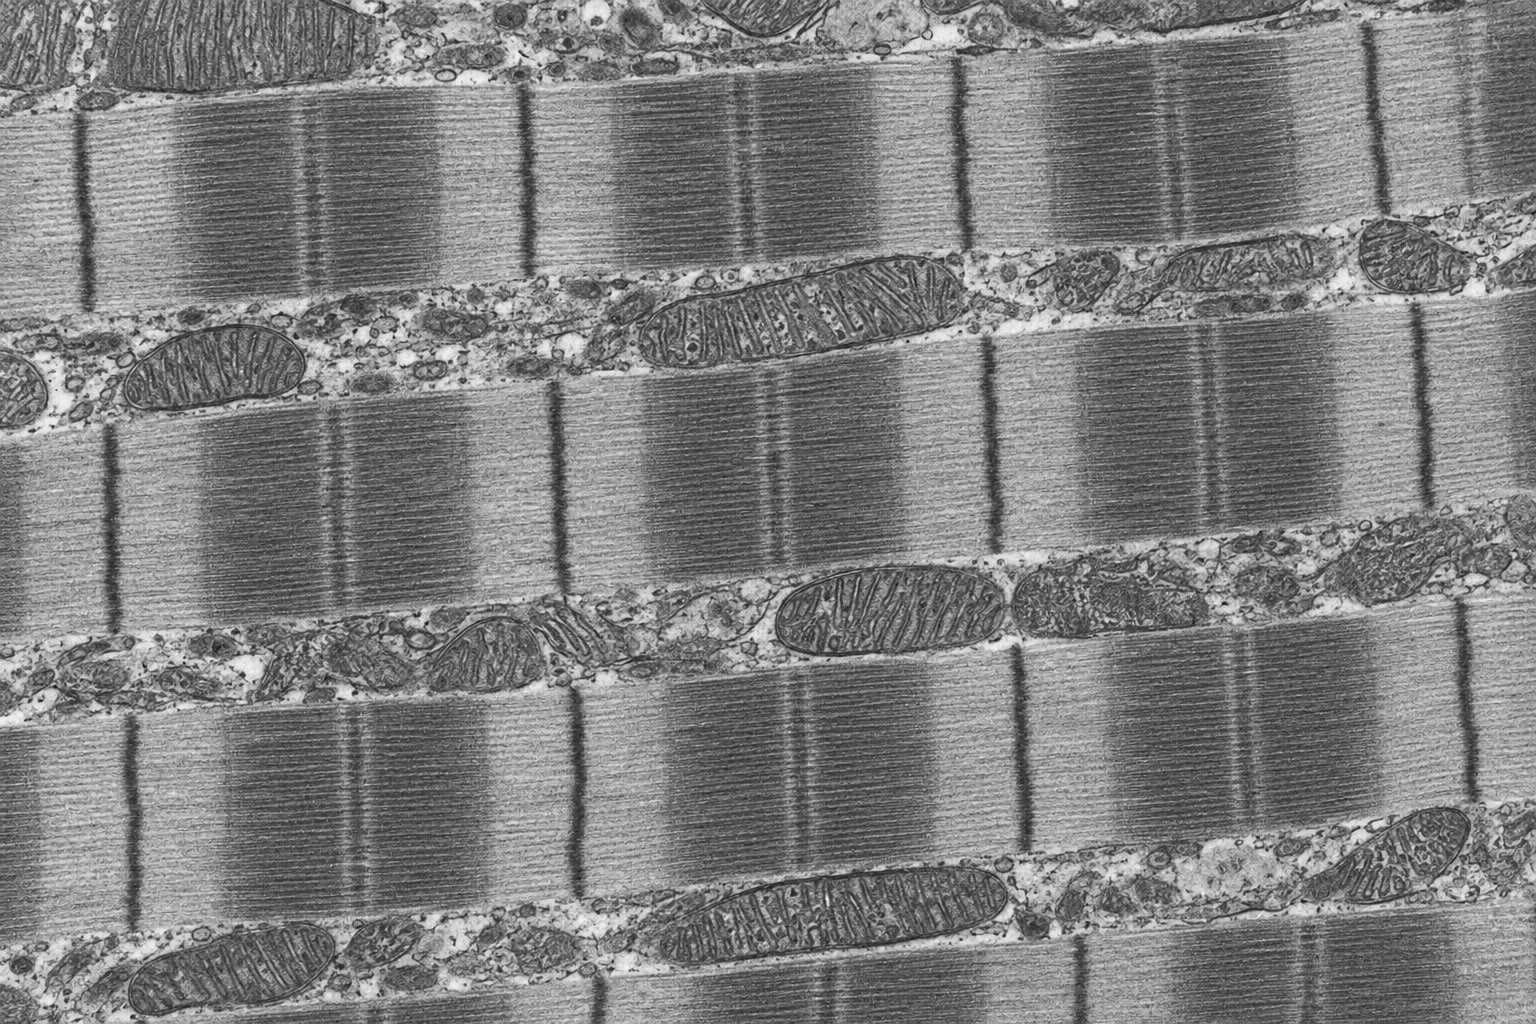
\includegraphics[width=0.6\linewidth]{images/book4/ai/b4-21-sarcomere-tem.jpg}

{\small \omterm{def:b2:cell-differentiation:fibre}{Miofibrilas} ao microscópio eletrônico: as bandas A de filamentos
grossos, as bandas I de filamentos finos cortadas pelas linhas Z, e as
mitocôndrias entre as fibrilas, que pagam o deslizamento.}
\end{omfigure}

\section{O motor}

\begin{proposition}[O ciclo das pontes cruzadas]\label{prop:b2:muscle-movement:crossbridge}
\index{ciclo das pontes cruzadas}\index{miosina}\index{ATP!na contração}
Cada filamento grosso está eriçado de cerca de trezentas \emph{cabeças
de miosina}, e cada cabeça é um motor que caminha ao longo da actina
num ciclo de quatro etapas. (1) Com ATP ligado, a cabeça está solta da
actina; ela hidrolisa o ATP em ADP e fosfato e se arma numa forma
tensionada, de alta energia. (2) A cabeça armada se liga a uma
subunidade de actina, formando uma \emph{ponte cruzada}. (3) O fosfato
é liberado e a cabeça volta bruscamente à sua forma relaxada, puxando o
filamento fino cerca de \qty{10}{nm} em direção ao centro do \omterm{def:b2:cell-differentiation:fibre}{sarcômero}
--- o \emph{golpe de força}; o ADP sai. (4) Um novo ATP se liga e a
cabeça solta a actina; sem ATP, ela não consegue soltar, e essa é a
rigidez da morte. O ciclo dura cerca de um vigésimo de segundo; uma
cabeça passa a maior parte dele solta, de modo que, a cada instante,
apenas uma fração das cabeças puxa, e um filamento que desliza depressa
nunca é largado. A força é a soma das trações das cabeças ligadas; o
encurtamento é a soma de seus passos, no máximo meio micrômetro por
\omterm{def:b2:cell-differentiation:fibre}{sarcômero} por ciclo; e a energia é um ATP por passo por cabeça, cerca de
\qty{50}{kJ/mol} --- \qty{8e-20}{J} por passo, dos quais a cabeça
converte até metade em trabalho.
\end{proposition}

\begin{omfigure}
\begin{tikzpicture}[every node/.style={font=\scriptsize}, >=stealth]
  \foreach \x/\lab/\ang/\att in {0/{1. ATP ligado:\\cabeça solta; ATP\\hidrolisado, cabeça armada}/60/0, 3.6/{2. a cabeça armada\\se liga à actina:\\ponte cruzada}/60/1, 7.2/{3. fosfato liberado:\\golpe de força,\\filamento puxado \qty{10}{nm}}/20/1, 10.8/{4. o ADP sai, um novo\\ATP se liga: a cabeça\\solta}/20/0} {
    \begin{scope}[xshift=\x cm]
      \draw[thick, omDef] (0,2.2) -- (2.8,2.2); \foreach \i in {0.2,0.6,...,2.6} \fill[omDef!50] (\i,2.2) circle (0.14);
      \draw[line width=3pt, omExo!80!black] (0,0.4) -- (2.8,0.4);
      \draw[very thick, omThm] (1.4,0.4) -- (1.4,1.0);
      \ifnum\att=1 \draw[very thick, omThm] (1.4,1.0) -- ++(\ang:1.15); \fill[omThm] (1.4,1.0) ++(\ang:1.15) circle (0.16); \else \draw[very thick, omThm] (1.4,1.0) -- ++(\ang:1.0); \fill[omThm] (1.4,1.0) ++(\ang:1.0) circle (0.16); \fi
      \node[below, align=center] at (1.4,0.15) {\lab};
    \end{scope}
  }
  \draw[->, thick, omDef] (7.9,2.55) -- (8.9,2.55); \node[omDef, above] at (8.4,2.6) {o filamento fino se move};
\end{tikzpicture}

{\small O \omterm{prop:b2:muscle-movement:crossbridge}{ciclo das pontes cruzadas}. Uma cabeça de miosina armada
(vermelho) se liga à actina (azul), libera o fosfato e puxa o filamento
fino em seu golpe de força, depois liga um ATP novo e solta.}
\end{omfigure}

\begin{theorem}[Força, velocidade e potência de um músculo]\label{thm:b2:muscle-movement:hill}
\index{curva força--velocidade}\index{potência muscular}
A força de um músculo cai à medida que ele encurta mais depressa,
porque, quanto mais rápido os filamentos deslizam, menos cabeças estão
ligadas a cada instante e mais delas são arrastadas além de seu golpe
antes de soltar. A relação de Hill a descreve:
\[
(F + a)(v + b) = (F_0 + a)\,b,
\]
em que $F_0$ é a força isométrica (com $v = 0$), $v_{\max} =
F_0 b/a$ a velocidade sem carga, e $a$ e $b$ são constantes
($a \approx
F_0/4$). A potência $Fv$ é nula nas duas extremidades e máxima a cerca
de um terço de $v_{\max}$ e um terço de $F_0$ --- e é por isso que um
ciclista troca de marcha e que a passada de um velocista tem uma
frequência preferida. Um músculo humano desenvolve cerca de
\qty{30}{N} por centímetro quadrado de seção transversal, encurta até
dez comprimentos por segundo e fornece uns \qty{100}{W} por quilograma
no seu melhor.
\end{theorem}
\begin{proof}
A curva de Hill é empírica (1938), medida em músculo isolado de rã como
a velocidade de encurtamento em função da carga que ele levanta; a
hipérbole se ajusta porque a fração de cabeças ligadas cai com a
velocidade de deslizamento e a força de cada cabeça ligada cai à medida
que ela é levada ao longo de seu golpe. Potência: com
$F = (F_0 + a)b/(v + b) - a$, $Fv$ é nula em
$v = 0$ e em $v_{\max}$; derivando, obtém-se o máximo em
$v = b(\sqrt{(F_0 + a)/a} - 1)$, que para $a = F_0/4$ é $v =
1.24\,b = 0.31\,v_{\max}$, onde $F = 0.31\,F_0$.
\end{proof}

\begin{omfigure}
\begin{tikzpicture}
\begin{axis}[
  width=0.7\linewidth, height=5.4cm,
  axis x line=bottom, axis y line=left,
  xmin=0, xmax=1.05, ymin=0, ymax=1.1,
  xlabel={velocidade de encurtamento $v/v_{\max}$}, ylabel={força $F/F_0$, potência (relativa)},
  xlabel style={font=\small, at={(axis description cs:0.5,-0.13)}, anchor=north},
  ylabel style={font=\small},
  tick label style={font=\small}, xtick={0,0.31,1}, xticklabels={0,0.31,1}, ytick={0,0.31,1}, yticklabels={0,0.31,1},
  legend style={font=\scriptsize, at={(0.97,0.95)}, anchor=north east, draw=none},
  clip=false,
]
\addplot[very thick, omDef, domain=0:1, samples=100] {(1.25*0.25)/(x+0.25) - 0.25};
\addlegendentry{força}
\addplot[very thick, omThm, domain=0:1, samples=100] {10.4*x*((1.25*0.25)/(x+0.25) - 0.25)};
\addlegendentry{potência (em escala)}
\draw[dashed, gray] (axis cs:0.31,0) -- (axis cs:0.31,1.0);
\end{axis}
\end{tikzpicture}

{\small A \omterm{thm:b2:muscle-movement:hill}{curva força--velocidade} de Hill ($a = F_0/4$) e a potência que
ela implica: a força cai à medida que o músculo encurta mais depressa, e
a potência atinge o máximo a cerca de um terço da velocidade máxima e
um terço da força isométrica.}
\end{omfigure}

\section{O interruptor: o cálcio}

\begin{proposition}[O acoplamento excitação--contração]\label{prop:b2:muscle-movement:coupling}
\index{acoplamento excitação--contração}\index{troponina}\index{tropomiosina}\index{retículo sarcoplasmático}
Em repouso, as cabeças de miosina não conseguem alcançar a actina: os
sítios de ligação do filamento fino estão cobertos pela
\emph{tropomiosina}, um bastão deitado no sulco da hélice de actina,
mantido ali pela \emph{troponina}. O interruptor é o cálcio. Um
\omterm{prop:b2:neurons-synapses:ap}{potencial de ação} na membrana da fibra desce pelos \omterm{def:b2:cell-differentiation:fibre}{túbulos T} até o
interior e, nas junções em que um \omterm{def:b2:cell-differentiation:fibre}{túbulo T} encontra o \omterm{def:b2:cell-differentiation:fibre}{retículo
sarcoplasmático}, abre os canais de liberação de cálcio do retículo; o
cálcio inunda as \omterm{def:b2:cell-differentiation:fibre}{miofibrilas}, subindo de \qty{0.1}{} a
\qty{10}{\micro mol/L} em um milissegundo, liga-se à troponina, e a
troponina desloca a tropomiosina dos sítios de ligação: as cabeças se
ligam, e a fibra se contrai enquanto o cálcio permanecer. Bombas do
retículo, queimando ATP, recolhem o cálcio em dezenas de
milissegundos; a tropomiosina volta a cobrir os sítios e a fibra relaxa.
O relaxamento é, assim, tão ativo quanto a contração, e um músculo
privado de ATP não consegue nem soltar suas cabeças nem bombear seu
cálcio --- é o \textit{rigor mortis}. No \omterm{def:b2:heart:anatomy}{coração}, o mesmo interruptor é
usado, mas com cálcio vindo de fora, pelos canais da própria membrana,
para desencadear a liberação, e é por isso que o \omterm{def:b2:heart:anatomy}{coração}, e não o
músculo esquelético, é sensível ao cálcio do \omterm{def:b2:blood-circulation:blood}{sangue}.
\end{proposition}

\begin{omfigure}
\begin{tikzpicture}[every node/.style={font=\scriptsize}, >=stealth]
  \node[draw, rounded corners, fill=omDef!15, align=center] (nerve) at (0,0) {impulso do\\nervo motor};
  \node[draw, rounded corners, fill=omDef!15, align=center] (nmj) at (3.0,0) {junção\\neuromuscular:\\acetilcolina};
  \node[draw, rounded corners, fill=omDef!15, align=center] (ap) at (6.2,0) {potencial de ação\\muscular, pelos\\túbulos T};
  \node[draw, rounded corners, fill=omThm!15, align=center] (ca) at (9.4,0) {Ca$^{2+}$ liberado\\pelo retículo\\sarcoplasmático};
  \node[draw, rounded corners, fill=omProp!20, align=center] (tn) at (12.6,0) {a troponina liga Ca$^{2+}$,\\a tropomiosina se desloca,\\as cabeças se ligam};
  \node[draw, rounded corners, fill=omExo!25, align=center] (off) at (9.4,-2.2) {as bombas devolvem o Ca$^{2+}$ (ATP);\\a tropomiosina volta a cobrir a actina:\\relaxamento};
  \draw[->, thick] (nerve) -- (nmj); \draw[->, thick] (nmj) -- (ap); \draw[->, thick] (ap) -- (ca); \draw[->, thick] (ca) -- (tn);
  \draw[->, thick] (ca) -- (off);
  \node[below, gray] at (1.5,-0.7) {\qty{0.6}{ms}}; \node[below, gray] at (4.6,-0.7) {\qty{1}{ms}}; \node[below, gray] at (7.8,-0.7) {\qty{1}{ms}};
\end{tikzpicture}

{\small Do impulso nervoso à força: a junção, o \omterm{prop:b2:neurons-synapses:ap}{potencial de ação}
próprio da fibra, a liberação do cálcio e a exposição dos sítios da
actina --- depois as bombas que encerram o processo.}
\end{omfigure}

\section{Comando e gradação}

\begin{definition}[A unidade motora]\label{def:b2:muscle-movement:motorunit}
\index{unidade motora}\index{abalo muscular}\index{tétano}\index{recrutamento}
Um \emph{\omterm{def:b2:neurons-synapses:neuron}{neurônio} motor} da medula espinal envia seu \omterm{def:b2:neurons-synapses:neuron}{axônio} a um
músculo e se ramifica para inervar de um punhado a mil fibras,
espalhadas pelo músculo; o \omterm{def:b2:neurons-synapses:neuron}{neurônio} e suas fibras formam uma
\emph{unidade motora}, a menor quantidade de força que o sistema nervoso
consegue comandar. Cada impulso do \omterm{def:b2:neurons-synapses:neuron}{neurônio} faz cada fibra da unidade
disparar uma vez e dar um \emph{abalo}: uma força que sobe em cerca de
\qty{30}{ms} e decai em \qty{100}{ms}, porque o pulso de cálcio é breve.
Impulsos em rápida sucessão fazem os abalos se somarem, pois o cálcio de
um ainda não foi bombeado quando chega o seguinte; a cerca de 30 a 50
impulsos por segundo, a força se funde num \emph{tétano} contínuo, de
três a cinco vezes o abalo. O sistema nervoso gradua a força de um
músculo de duas maneiras: pela \emph{frequência} com que cada unidade
dispara e pelo \emph{número} de unidades que recruta --- as unidades
pequenas, lentas e resistentes à fadiga primeiro (o \emph{princípio do
tamanho}), as grandes e rápidas por último, apenas para os maiores
esforços. Um músculo em uso comum nunca está, portanto, totalmente
ativo: uma fração de suas unidades dispara, em rodízio, e as demais
descansam.
\end{definition}

\begin{omfigure}
\begin{tikzpicture}
\begin{axis}[
  width=0.82\linewidth, height=5.4cm,
  axis x line=bottom, axis y line=left,
  xmin=0, xmax=1.0, ymin=0, ymax=4.2,
  xlabel={tempo (s)}, ylabel={força (abalo $=$ 1)},
  xlabel style={font=\small, at={(axis description cs:0.5,-0.13)}, anchor=north},
  ylabel style={font=\small},
  tick label style={font=\small}, xtick={0,0.2,0.4,0.6,0.8,1}, ytick={0,1,2,3,4},
  clip=false,
]
% single twitch
\addplot[very thick, omDef, domain=0:0.2, samples=60] {(x<0.02)*0 + (x>=0.02)*4.5*(x-0.02)*exp(-(x-0.02)/0.03)*4.1};
% summation at 10 Hz
\addplot[very thick, omProp, domain=0.25:0.62, samples=200] {(x>=0.25)*4.5*4.1*(x-0.25)*exp(-(x-0.25)/0.03) + (x>=0.33)*4.5*4.1*(x-0.33)*exp(-(x-0.33)/0.03) + (x>=0.41)*4.5*4.1*(x-0.41)*exp(-(x-0.41)/0.03) + (x>=0.49)*4.5*4.1*(x-0.49)*exp(-(x-0.49)/0.03)};
% tetanus at 50 Hz
\addplot[very thick, omThm, domain=0.66:0.98, samples=100] {3.8*(1-exp(-(x-0.66)/0.06))};
\node[font=\scriptsize, anchor=west] at (axis cs:0.09,0.7) {um impulso: abalo};
\node[font=\scriptsize, anchor=south] at (axis cs:0.44,2.2) {\qty{12}{Hz}: somação};
\node[font=\scriptsize, anchor=south] at (axis cs:0.82,3.85) {\qty{50}{Hz}: tétano fundido};
\end{axis}
\end{tikzpicture}

{\small A gradação da força pela frequência. Um único impulso dá um
\omterm{def:b2:muscle-movement:motorunit}{abalo}; impulsos a uma dúzia por segundo se somam numa força ondulante;
a cinquenta por segundo, a força se funde num \omterm{def:b2:muscle-movement:motorunit}{tétano} várias vezes maior
que o \omterm{def:b2:muscle-movement:motorunit}{abalo}.}
\end{omfigure}

\begin{proposition}[Os reflexos e a medula espinal]\label{prop:b2:muscle-movement:reflex}
\index{arco reflexo}\index{fuso muscular}\index{reflexo de estiramento}\index{inibição recíproca}
O \omterm{def:b2:neurons-synapses:neuron}{neurônio} motor é a \emph{via final comum}: todo comando, do córtex ou
de um reflexo, termina nele. O circuito mais simples é o \emph{\omterm{prop:b2:muscle-movement:reflex}{reflexo
de estiramento}} do \cref{ch:b2:neurons-synapses}: terminações sensitivas enroladas em torno
de fibras especiais dentro do músculo, os \emph{\omterm{prop:b2:muscle-movement:reflex}{fusos musculares}},
disparam quando o músculo é estirado, excitam os \omterm{def:b2:neurons-synapses:neuron}{neurônios} motores do
mesmo músculo por meio de uma única \omterm{def:b2:neurons-synapses:synapse}{sinapse} e inibem os do antagonista
por meio de um interneurônio (\emph{\omterm{prop:b2:muscle-movement:reflex}{inibição recíproca}}), de modo que o
músculo resiste ao estiramento --- a base da postura, pois toda
oscilação é um estiramento de algum músculo. Um segundo receptor, o
órgão tendinoso, dispara quando a força do músculo é alta e inibe seus
próprios \omterm{def:b2:neurons-synapses:neuron}{neurônios} motores: uma válvula de segurança. A retirada diante
de um estímulo doloroso é um reflexo de várias \omterm{def:b2:neurons-synapses:synapse}{sinapses} que flexiona o
membro e, do outro lado, estende o outro membro para que você não caia.
E o encéfalo não comanda músculos, mas movimentos: o córtex envia um
plano, o cerebelo o corrige com base no que os fusos informam, os
núcleos da base o liberam, e os circuitos da medula espinal, que
conseguem produzir sozinhos um ritmo de marcha, o executam --- o assunto
do volume do Ano 3.
\end{proposition}

\begin{omfigure}
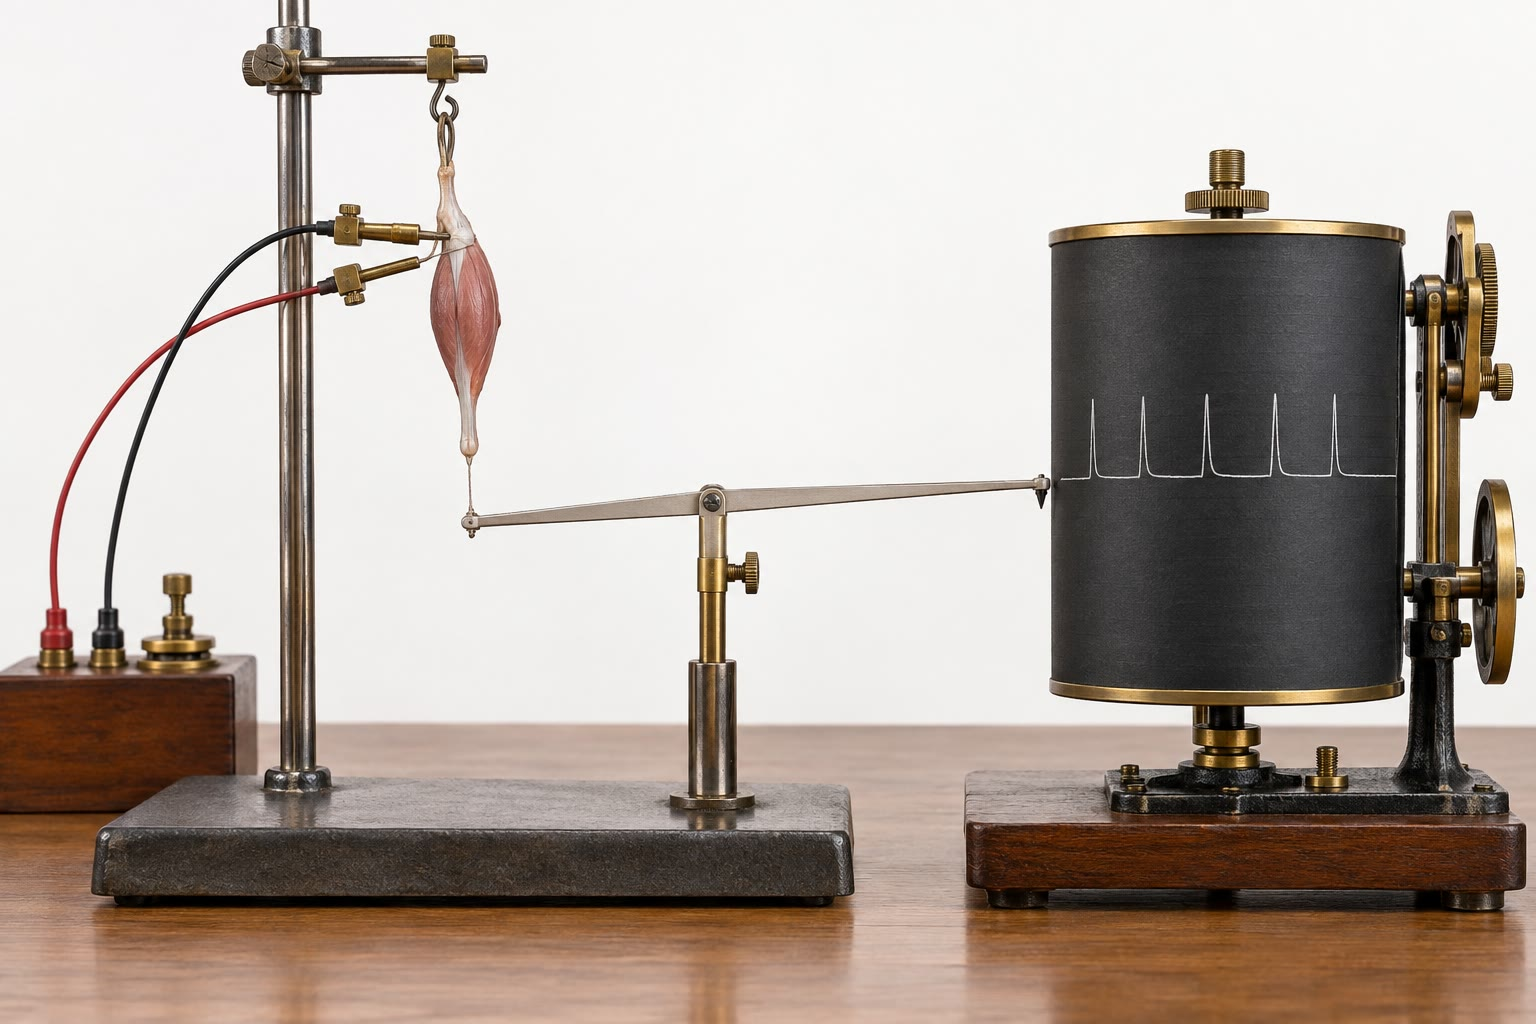
\includegraphics[width=0.44\linewidth]{images/book4/ai/b4-21-frog-muscle-prep.jpg}\hspace{0.04\linewidth}
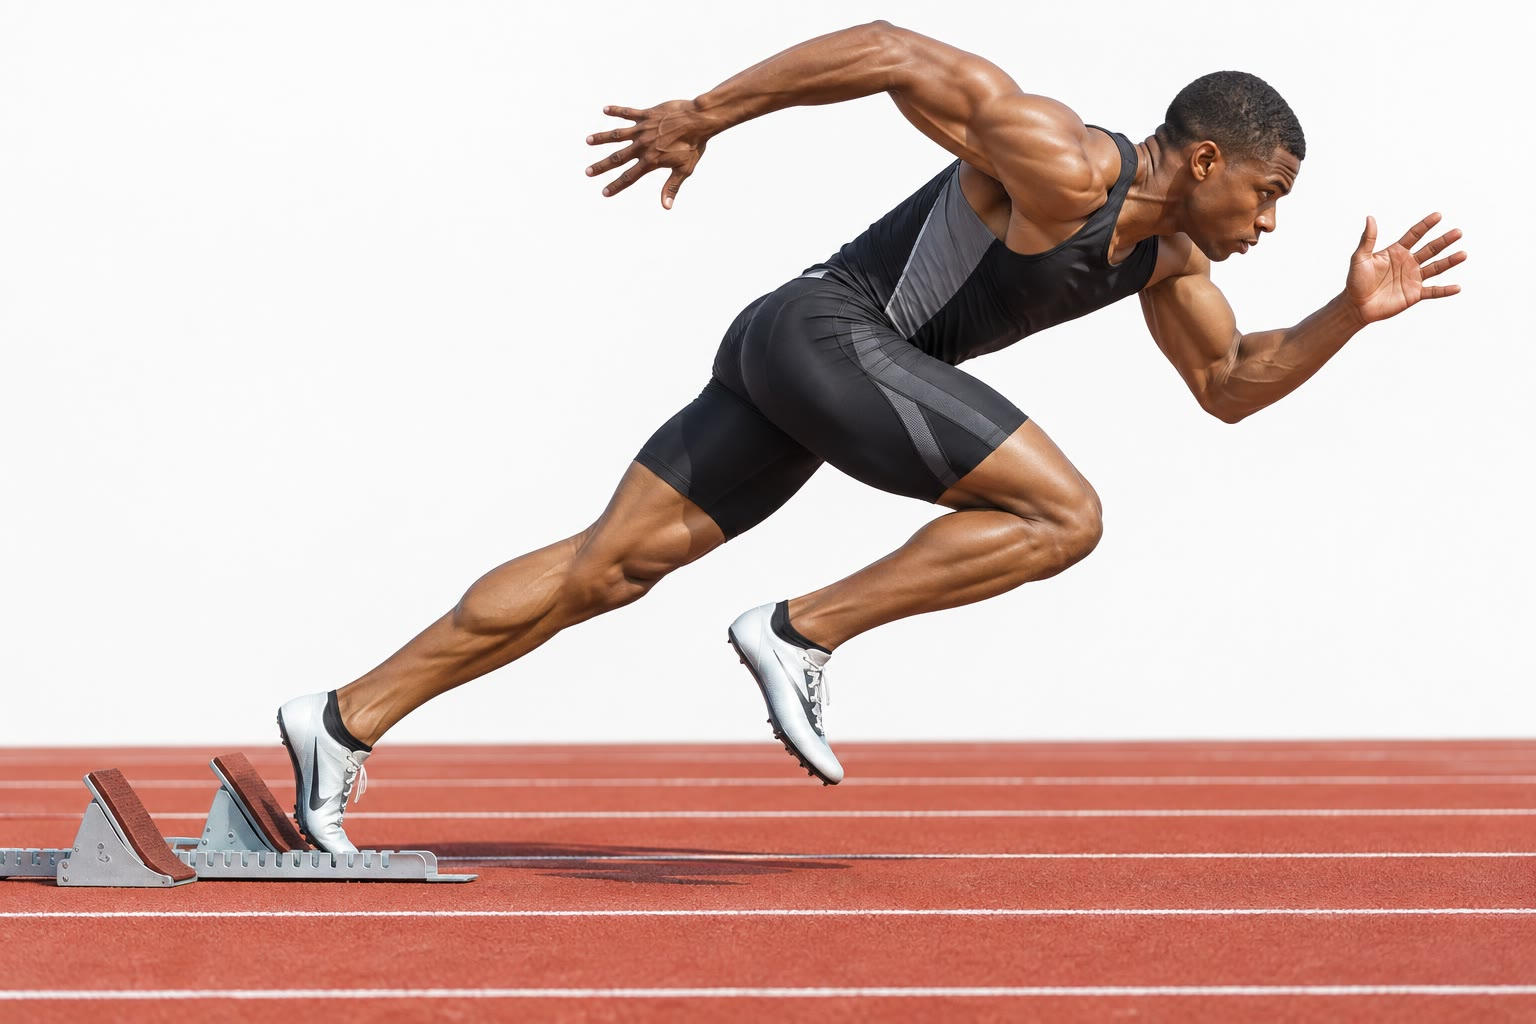
\includegraphics[width=0.44\linewidth]{images/book4/ai/b4-21-sprinter.jpg}

{\small À esquerda: a preparação clássica --- um músculo de rã, seu
nervo, eletrodos de estimulação e uma alavanca que escreve num tambor
enegrecido de fuligem ---, com a qual o \omterm{def:b2:muscle-movement:motorunit}{abalo}, a somação e o \omterm{def:b2:muscle-movement:motorunit}{tétano} foram
registrados pela primeira vez. À direita: a mesma fisiologia em pleno
esforço.}
\end{omfigure}

\section{Combustível e fadiga}

\begin{proposition}[Pagar pelo trabalho]\label{prop:b2:muscle-movement:energy}
\index{fosfocreatina}\index{fadiga muscular}\index{débito de oxigênio}
Uma fibra contém ATP para um ou dois segundos de esforço máximo. A
primeira reserva é a \emph{\omterm{prop:b2:muscle-movement:energy}{fosfocreatina}}, que refosforila o ADP em
milissegundos e dura uns dez segundos --- o combustível do velocista. A
segunda é a \emph{glicólise} do glicogênio da fibra, sem oxigênio, que
fornece dois ATP por glicose e lactato: rápida, suficiente para um ou
dois minutos, e autolimitada à medida que ácido e fosfato se acumulam.
A terceira é o metabolismo \emph{oxidativo} da glicose e dos ácidos
graxos nas mitocôndrias, trinta ATP por glicose, limitado apenas pelo
oxigênio que o \omterm{def:b2:blood-circulation:blood}{sangue} fornece (\cref{ch:b2:blood-pressure}): a maratona. As fibras
glicolíticas rápidas dependem das duas primeiras e se cansam em um
minuto; as fibras oxidativas lentas, vermelhas de mioglobina e repletas
de mitocôndrias, funcionam durante horas. A \emph{fadiga} num esforço
curto não é o esgotamento do ATP --- que deixaria o músculo rígido ---,
mas o acúmulo de fosfato e de prótons, que enfraquecem as pontes
cruzadas e a liberação de cálcio; num esforço longo, é o esgotamento do
glicogênio e, por fim, da vontade. Após o esforço, o músculo paga seu
\emph{\omterm{prop:b2:muscle-movement:energy}{débito de oxigênio}}: restaura a \omterm{prop:b2:muscle-movement:energy}{fosfocreatina}, reconverte o
lactato (no fígado) e reabastece suas reservas, respirando com força
durante minutos depois de parar.
\end{proposition}

\begin{example}[Cem metros]\label{ex:b2:muscle-movement:sprint}
Dez segundos de esforço máximo de \qty{20}{kg} de músculos das pernas a
\qty{100}{W/kg} são \qty{2}{kW} de potência mecânica e, com
\qty{25}{\%} de eficiência, \qty{8}{kW} de renovação de ATP --- cerca de
\qty{160}{mmol} de ATP por segundo, ou \qty{800}{g} de ATP na corrida.
O músculo contém cerca de cinquenta gramas; a \omterm{prop:b2:muscle-movement:energy}{fosfocreatina} fornece os primeiros
cinco segundos, a glicólise o restante, e a velocista termina com um
lactato de \qty{15}{mmol/L} no \omterm{def:b2:blood-circulation:blood}{sangue} e um débito que ela paga no quarto
de hora seguinte. Uma maratonista a \qty{300}{W} durante duas horas
queima \qty{2}{MJ} de trabalho, \qty{8}{MJ} de combustível --- um
quilograma de glicogênio e gordura ---, com oxigênio fornecido a
\qty{4}{L/min} durante todo o percurso, e o muro que ela encontra no
trigésimo quilômetro é o fundo de seu glicogênio.
\end{example}

\section{Exercícios}

\begin{exercise}[$\star$]\label{exo:b2:muscle-movement:1}
Enuncie o mecanismo dos \omterm{prop:b2:muscle-movement:sliding}{filamentos deslizantes} e diga quais bandas do
\omterm{def:b2:cell-differentiation:fibre}{sarcômero} mudam na contração e quais não mudam.
\end{exercise}

\begin{exercise}[$\star$]\label{exo:b2:muscle-movement:2}
Dê as quatro etapas do \omterm{prop:b2:muscle-movement:crossbridge}{ciclo das pontes cruzadas} e o papel do ATP em
cada uma. Por que um músculo sem ATP fica rígido?
\end{exercise}

\begin{exercise}[$\star$]\label{exo:b2:muscle-movement:3}
Liste os eventos que vão de um impulso do nervo motor à ligação das
cabeças de miosina, com o tempo que cada um leva.
\end{exercise}

\begin{exercise}[$\star$]\label{exo:b2:muscle-movement:4}
Defina \omterm{def:b2:muscle-movement:motorunit}{unidade motora}, \omterm{def:b2:muscle-movement:motorunit}{abalo} e \omterm{def:b2:muscle-movement:motorunit}{tétano}, e dê as duas maneiras pelas quais
o sistema nervoso gradua a força.
\end{exercise}

\begin{exercise}[$\star\star$]\label{exo:b2:muscle-movement:5}
Um \omterm{def:b2:cell-differentiation:fibre}{sarcômero} de \qty{2.4}{\micro m} encurta para \qty{2.0}{\micro m} em
\qty{50}{ms}. Calcule a velocidade de deslizamento dos filamentos finos
em relação aos grossos e, com um passo de \qty{10}{nm}, o número de
ciclos que cada cabeça ligada precisa realizar por segundo.
\end{exercise}

\begin{exercise}[$\star\star$]\label{exo:b2:muscle-movement:6}
Uma fibra de \qty{10}{cm} tem \num{40000} \omterm{def:b2:cell-differentiation:fibre}{sarcômeros} em série e encurta
\qty{20}{\%} em \qty{0.1}{s}. Calcule sua velocidade de encurtamento em
comprimentos por segundo e em metros por segundo, e a velocidade de cada
\omterm{def:b2:cell-differentiation:fibre}{sarcômero}.
\end{exercise}

\begin{exercise}[$\star\star$]\label{exo:b2:muscle-movement:7}
Com a relação de Hill e $a = F_0/4$, $v_{\max} = 10$ comprimentos por
segundo, calcule a força (como fração de $F_0$) a 1, 3 e 6 comprimentos
por segundo, e a potência em cada caso. Onde a potência é máxima?
\end{exercise}

\begin{exercise}[$\star\star$]\label{exo:b2:muscle-movement:8}
Um quadríceps de \qty{80}{cm^2} de seção transversal a
\qty{30}{N/cm^2}: calcule sua força isométrica máxima. Ele age a
\qty{5}{cm} da articulação do joelho sobre uma alavanca cujo pé fica a
\qty{45}{cm} da articulação: que força o pé consegue exercer?
\end{exercise}

\begin{exercise}[$\star\star$]\label{exo:b2:muscle-movement:9}
O pulso de cálcio de um \omterm{def:b2:muscle-movement:motorunit}{abalo} dura \qty{30}{ms}. Explique por que
impulsos a \qty{10}{Hz} dão uma força ondulante e a \qty{50}{Hz} um
\omterm{def:b2:muscle-movement:motorunit}{tétano} contínuo, e por que a força tetânica supera a do \omterm{def:b2:muscle-movement:motorunit}{abalo}.
\end{exercise}

\begin{exercise}[$\star\star\star$]\label{exo:b2:muscle-movement:10}
Os \qty{20}{kg} de músculos das pernas de uma velocista fornecem
\qty{2}{kW} durante \qty{10}{s} com \qty{25}{\%} de eficiência. Calcule
o ATP usado (\qty{50}{kJ/mol}), a \omterm{prop:b2:muscle-movement:energy}{fosfocreatina} necessária para cobrir
os primeiros \qty{5}{s} e a glicose fermentada para cobrir o restante
(2 ATP por glicose). Que concentração de lactato isso produz em
\qty{40}{L} de água corporal?
\end{exercise}

\begin{exercise}[$\star\star\star$]\label{exo:b2:muscle-movement:11}
Preveja o efeito sobre a contração de: um fármaco que bloqueia o canal
de liberação de cálcio do retículo; um que bloqueia sua bomba; uma
\omterm{def:b2:genome-diversification:mutation}{mutação} que torna a troponina insensível ao cálcio; a remoção do cálcio
do \omterm{def:b2:blood-circulation:blood}{sangue}, para o músculo esquelético e para o \omterm{def:b2:heart:anatomy}{coração}.
\end{exercise}

\begin{exercise}[$\star\star\star$]\label{exo:b2:muscle-movement:12}
``Um músculo é uma máquina que converte energia química em força com a
eficiência de um bom motor e o controle de um computador.'' Discuta a
eficiência (de um quarto a metade), o que a limita, e o que as duas
maneiras de graduar a força do sistema nervoso proporcionam que um
simples interruptor não proporcionaria.
\end{exercise}

\section{Problema: A fisiologia de um salto}

\begin{problem}[{Problema de fim de semana --- um salto vertical parado
analisado do sarcômero à decolagem: o deslizamento, as pontes cruzadas,
o interruptor de cálcio, o limite força--velocidade, as unidades motoras
e o combustível, até o número de golpes das pontes cruzadas, a força na
velocidade de decolagem e o ATP que o salto custa}]
\label{pb:b2:muscle-movement:1}
Uma pessoa de \qty{70}{kg} salta \qty{40}{cm} na vertical, elevando o
centro de massa do corpo em \qty{0.4}{m} durante um impulso de
\qty{0.3}{s}. Os extensores das pernas (\qty{20}{kg} de músculo) têm uma
seção transversal combinada de \qty{500}{cm^2} a \qty{30}{N/cm^2}; suas
fibras têm \qty{12}{cm} de comprimento (\num{48000} \omterm{def:b2:cell-differentiation:fibre}{sarcômeros}) e
encurtam \qty{4}{cm} durante o impulso; as articulações multiplicam o
encurtamento do músculo por \num{10} no pé e dividem sua força pelo
mesmo fator. $v_{\max} = 8$ comprimentos por segundo, $a = F_0/4$. Cada
filamento grosso tem \num{300} cabeças de miosina; há $6\times
10^{10}$ filamentos grossos por centímetro quadrado de músculo; um golpe
mede \qty{10}{nm} e custa um ATP (\qty{8e-20}{J}, \qty{50}{kJ/mol});
eficiência de \qty{40}{\%}. O músculo contém \qty{5}{mmol/kg} de ATP e
\qty{20}{mmol/kg} de \omterm{prop:b2:muscle-movement:energy}{fosfocreatina}. As fibras têm \qty{60}{\micro
m} de diâmetro. \omterm{def:b2:muscle-movement:motorunit}{Unidades motoras}: \num{800} por grupo muscular, de
\num{50} a \num{2000} fibras cada.

\medskip
\noindent\textbf{Parte I --- A mecânica.}
\begin{enumerate}
  \item Calcule a velocidade de decolagem necessária para subir
        \qty{40}{cm} ($v^{2} = 2gh$) e a energia cinética na decolagem.
  \item Calcule a força média que as pernas exercem sobre o chão durante
        o impulso (o trabalho ao longo de \qty{0.4}{m} é igual à energia
        cinética mais o trabalho contra a gravidade), e compare com o
        peso.
  \item Calcule a força isométrica máxima dos extensores e, com a razão
        de alavanca de 10, a força máxima que ela poderia dar no pé.
  \item Calcule a velocidade de encurtamento das fibras em comprimentos
        por segundo e como fração de $v_{\max}$.
  \item Com a relação de Hill, calcule a força disponível nessa
        velocidade como fração de $F_0$, e a força no pé que ela dá. O
        músculo sozinho consegue realizar o salto? De onde vem o
        restante?
  \item Calcule a potência mecânica média durante o impulso e a potência
        por quilograma de extensor.
\end{enumerate}

\medskip
\noindent\textbf{Parte II --- As pontes cruzadas.}
\begin{enumerate}[resume]
  \item Quanto cada \omterm{def:b2:cell-differentiation:fibre}{sarcômero} encurta, e quantos golpes de \qty{10}{nm}
        precisam ser dados ao longo de cada meio \omterm{def:b2:cell-differentiation:fibre}{sarcômero} para deslizar
        seus filamentos nessa distância?
  \item Calcule a velocidade de deslizamento em cada meio \omterm{def:b2:cell-differentiation:fibre}{sarcômero} e o
        número de golpes por segundo que uma cabeça faria se ficasse
        ligada continuamente.
  \item Calcule o número de cabeças de miosina nos extensores.
  \item Calcule o trabalho realizado pelo próprio músculo (sua força na
        velocidade do salto vezes seu encurtamento), o trabalho por
        golpe com \qty{40}{\%} de eficiência e o número de golpes
        necessários.
  \item Quantos golpes isso representa por cabeça, em comparação com o
        número disponível segundo a questão 7? Comente a reserva.
  \item Calcule o ATP consumido pelo salto, em mols e em gramas
        (\qty{507}{g/mol}), e confira a eficiência a partir da energia
        desse ATP.
\end{enumerate}

\medskip
\noindent\textbf{Parte III --- O interruptor e o comando.}
\begin{enumerate}[resume]
  \item O impulso dura \qty{0.3}{s} e o pulso de cálcio de um impulso
        nervoso, \qty{30}{ms}. Que frequência de disparo mantém as
        fibras em \omterm{def:b2:muscle-movement:motorunit}{tétano}, e quantos impulsos cada \omterm{def:b2:neurons-synapses:neuron}{neurônio} motor envia?
  \item O cálcio livre sobe de \qty{0.1}{} a \qty{10}{\micro
        mol/L} numa fibra de \qty{5e-10}{L}. Quantos íons de cálcio
        livres isso representa, e quantos ciclos da bomba (dois íons por
        ATP) custa recolhê-los?
  \item Calcule o número de fibras dos extensores e o ATP das pontes
        cruzadas por fibra por impulso, e compare com o custo de
        bombeamento da questão 14. O custo real do bombeamento é de cerca
        de um quarto do ATP do músculo: o que o cálcio livre subestima?
  \item O sistema nervoso recruta as unidades pelo tamanho. Para o
        salto, que unidades são recrutadas, e em que ordem? Que fração
        das \num{800} um passo suave usaria?
  \item Explique por que a força pode ser graduada finamente num esforço
        baixo e apenas grosseiramente perto do máximo.
  \item Uma pessoa sob um fármaco que bloqueia pela metade a \omterm{prop:b2:neurons-synapses:integration}{junção
        neuromuscular}: preveja o \omterm{def:b2:muscle-movement:motorunit}{abalo}, o \omterm{def:b2:muscle-movement:motorunit}{tétano} e o salto.
\end{enumerate}

\medskip
\noindent\textbf{Parte IV --- O combustível.}
\begin{enumerate}[resume]
  \item Calcule o ATP armazenado nos extensores e compare com o consumo
        do salto.
  \item Calcule a reserva de \omterm{prop:b2:muscle-movement:energy}{fosfocreatina} e o número de saltos que ela
        poderia pagar.
  \item Dez saltos seguidos: que combustível assume, e o que se acumula?
  \item O \omterm{def:b2:blood-circulation:blood}{sangue} consegue fornecer \qty{2}{L} de oxigênio por minuto aos
        extensores (6 ATP por $\mathrm{O_2}$). Que renovação de ATP a
        potência do salto exige, e que suprimento de oxigênio isso
        exigiria? Conclua.
  \item Após os saltos, a pessoa respira com força durante um minuto.
        Calcule o oxigênio necessário para ressintetizar a \omterm{prop:b2:muscle-movement:energy}{fosfocreatina}
        e o ATP usados (\qty{6}{ATP} por molécula de $\mathrm{O_2}$) e
        compare com o consumo de repouso de \qty{250}{mL/min}.
  \item Por que o músculo de quem salta não entra em rigidez, embora o
        ATP seja renovado a esse ritmo?
  \item Enuncie o resultado: os golpes por meio \omterm{def:b2:cell-differentiation:fibre}{sarcômero}, a fração de
        força na velocidade do salto e o ATP que o salto custa.
\end{enumerate}
\end{problem}
